\documentclass{article}
\usepackage{caption}
\usepackage{subcaption}
\usepackage{amsmath}
\usepackage{amssymb}
\usepackage{mathtools}
\usepackage[margin=0.75in]{geometry}
\usepackage{fancyhdr}
\usepackage{xcolor}
\usepackage{tikz}
\usetikzlibrary{backgrounds}
\usetikzlibrary{calc}
\usepackage[normalem]{ulem} % for strike through text
\setlength{\headheight}{0in}

\newcommand{\problemsep}{\leavevmode\\[0.05in] \rule[\baselineskip/4]{\textwidth}{1pt} \\[0.005in] \rule[\baselineskip]{\textwidth}{1pt}\vspace{-\baselineskip}\leavevmode\\[0.05in]}
\newcommand{\statementsep}{\leavevmode\\[0.005in] \rule[\baselineskip/4]{\textwidth}{0.4pt}\leavevmode\\[0.005in]}
\pagestyle{fancy}
\rhead{\today}
\lhead{Daniel Mortensen}
\chead{Homework 4}

\begin{document}
\noindent\underline{Problem 1}: Consider, again, the Petersen graph; thatis, the graph from HW5.2: $G = (V,E), V=\{2-\text{sets of } [5]\}$, vertices adjacent if and only if they are disjoint. Define $\tau(H)$ to be the number of spanning trees of graph $H$. 
\begin{enumerate}
	\item Compute $\tau(G)$
	\item Let $e$ be any edge of $G$, and define $G'$ to be $g - e$  ($G$ with the edge $e$ deleted); find all possible values of $\tau(G')$.
	\item Let $G''$ be $G$ with two edges deleted. Determine all possible values of $\tau(G'')$.
	\item Recall that we proved this in class: {\it The maximum distance between anypair of vertices of $G$ is 2}. Please prove this using Theorem A.
\end{enumerate}
\statementsep
\begin{enumerate}
	\item We compute $\tau(G)$ as the determinant of the laplacian of the Petersen graph with one column/row removed. The laplacian of the Petersen graph is:
		\begin{equation*}
			\begin{tabular}{c | c | c | c | c |c | c | c | c | c | c |}
				   & 1,2 & 1,3 & 1,4 & 1,5 & 2,3 & 2,4 & 2,5 & 3,4 & 3,5 & 4,5 \\ \hline 
				1,2& 3   & 0   & 0   & 0   & 0   & 0   & 0   & 1   & 1   & 1   \\ \hline
				1,3& 0   & 3   & 0   & 0   & 1   & 1   & 0   & 0   & 0   & 1   \\ \hline
				1,4& 0   & 0   & 3   & 0   & 1   & 0   & 1   & 0   & 1   & 0   \\ \hline
				1,5& 0   & 0   & 0   & 3   & 1   & 1   & 0   & 1   & 0   & 0   \\ \hline
				2,3& 0   & 0   & 1   & 1   & 3   & 0   & 0   & 0   & 0   & 1   \\ \hline
				2,4& 0   & 1   & 0   & 1   & 0   & 3   & 0   & 0   & 1   & 0   \\ \hline
				2,5& 0   & 1   & 1   & 0   & 0   & 0   & 3   & 1   & 0   & 0   \\ \hline
				3,4& 1   & 0   & 0   & 1   & 0   & 0   & 1   & 3   & 0   & 0   \\ \hline
				3,5& 1   & 0   & 1   & 0   & 0   & 1   & 0   & 0   & 3   & 0   \\ \hline
				4,5& 1   & 1   & 0   & 0   & 1   & 0   & 0   & 0   & 0   & 3   \\ \hline
			\end{tabular}
		\end{equation*}
		As the Petersen graph is not directed (otherwise the non-diagonal elements would the negative of their counterparts from the adjacency matrix).
	\item In this section we compute $\tau(G')$. First, note that the 
\end{enumerate}
In this proof, we will derive expressions for the number of edges and vertices and then use Euler's Identity to solve for the number of faces in the resulting graph. \\
Each edge is uniquely defined by it's vertex end points, so that each edge creates two vertex degrees. Therefore, the number of edges can be computed by
\begin{equation*}
	\text{nEdge} = \frac{1}{2}\sum_{v \in V(G)} \text{deg}(v)
\end{equation*}
where deg$(v)$ is the degree of a vertex. In the pizza cutter scenario, the exterior vertices will have one degree for each edge that connects them to another exterior edge and two more that connect it to the edges on either side which make up the 'crust'. The other vertices we will call 'interior' vertices which are formed by the intersection of the `lasers'. Because each interior vertex is uniquely defined by two lasers (consisting of four vertices), then the degree of each interior point is four. Furthermore, the number of interior points is defined as ${n \choose 4}$ as there is one interior point for each unique four-set of exerior points. So the total number of vertex degrees can be computed as
\begin{equation*}
	\text{nDegree} = n(n - 1 + 2) + 4{n \choose 4}
\end{equation*}
and consequently, the number of edges is 
\begin{equation*}\begin{aligned}
	\text{nEdge} &= \frac{n(n + 1)}{2} + 2{n\choose 4} \\
			     &= \frac{n(n - 1) + 2n}{2} + 2{n\choose 4} \\
				 &= {n \choose 1} + {n \choose 2} + 2 {n\choose 4}.
\end{aligned}\end{equation*}
Next, the number of edges is computed as $n + {n \choose 4}$ as there are $n$ vertices around the crust and each intersection is uniquely defined by four exterior points. Next, we use Euler's identity so that
\begin{equation*}\begin{aligned}
	n - e + f = 2 & \implies \left ({n \choose 1} + {n \choose 4} \right ) - \left ( {n \choose 1} + {n \choose 2} + 2{n\choose 4} \right) + f = 2 \\
				  & \implies -{n \choose 2} - {n \choose 4} + f = 2 \\
				  & \implies f = {n \choose 2} + {n \choose 4} + 2.
\end{aligned}\end{equation*}
However, this also includes the space outside the `pizza', therefore, the total number of pizza slices is 
\begin{equation*}\begin{aligned}
\text{nSlices} &= {n \choose 2} + {n \choose 4} + 1 \\
			   &= {n \choose 0} + {n \choose 2} + {n \choose 4}  \\
			   &= \sum_{i = 0}^2 {n \choose 2i}
\end{aligned}\end{equation*}
\problemsep
\noindent\underline{Problem 2}: 
Please prove that no tournament with exactly $4$ vertices is such that every 
vertex is a queen.
\statementsep
This proof will be given by way of contradiction.  Assume a scenario with four vertices where each vertex is a queen and label the vertices $a,b,c,d$ respectively. If vertex $a$ never wins, then it is not a queen, therefore the minimum number of rounds it may win and still be a queen is $1$. Furthermore we can assume that at least one vertex will only win $1$ round as there are six games and only four vertices. Therefore, without loss of generality, let $a$ be a vertex that only wins one round. If $a$ is a queen, then the vertex which lost to $a$ must win against every other vertex. In this example, let $a$ win against $b$, and $b$ win against all other vertices such that
\begin{center}
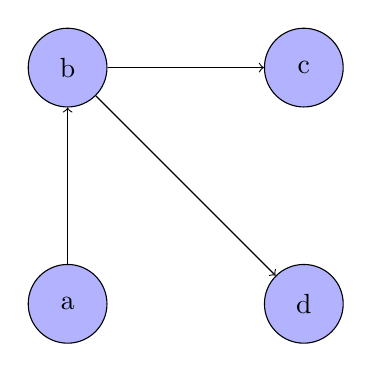
\begin{tikzpicture}[every node/.style={circle, draw=black, fill=blue!30, minimum size=1cm}]
	\node(a) at (0,0){a};
	\node(b) at (0,3){b};
	\node(c) at (3,3){c};
	\node(d) at (3,0){d};
	\draw[->] (a) -- (b);
	\draw[->] (b) -- (c);
	\draw[->] (b) -- (d);
\end{tikzpicture}
\end{center}
If vertex $c$ loses to $a$, then its path to $a$ would have to go through $d$, and would mean that it's path to $b$ is more than two, therefore $c$ must beat $a$. If $c$ loses to $d$, then it won't have a path to $d$, so $c$ must beat $d$ as well, yielding
\begin{center}
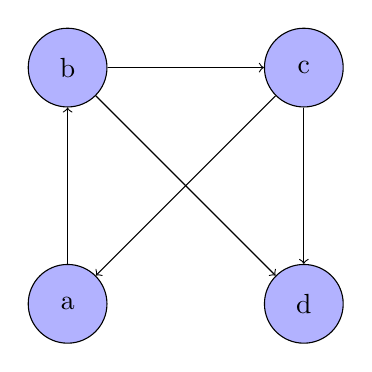
\begin{tikzpicture}[every node/.style={circle, draw=black, fill=blue!30, minimum size=1cm}]
	\node(a) at (0,0){a};
	\node(b) at (0,3){b};
	\node(c) at (3,3){c};
	\node(d) at (3,0){d};
	\draw[->] (a) -- (b);
	\draw[->] (b) -- (c);
	\draw[->] (b) -- (d);
	\draw[->] (c) -- (d);
	\draw[->] (c) -- (a);
\end{tikzpicture}
\end{center}
however, we assumed at the beginning that $a$ only won a single round, therefore $d$ must beat $a$.
\begin{center}
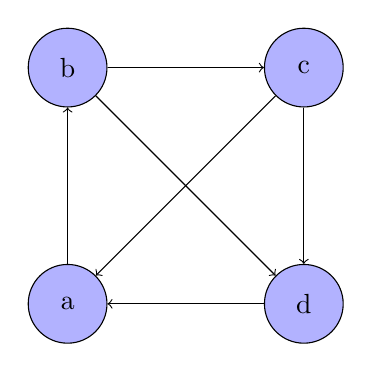
\begin{tikzpicture}[every node/.style={circle, draw=black, fill=blue!30, minimum size=1cm}]
	\node(a) at (0,0){a};
	\node(b) at (0,3){b};
	\node(c) at (3,3){c};
	\node(d) at (3,0){d};
	\draw[->] (a) -- (b);
	\draw[->] (b) -- (c);
	\draw[->] (b) -- (d);
	\draw[->] (c) -- (d);
	\draw[->] (c) -- (a);
	\draw[->] (d) -- (a);
\end{tikzpicture}
\end{center}
Upon inspection, the path from $d$ to $c$ is larger than two so that $d$ is not a queen which contradicts the original assumption that all vertices are queens.
\problemsep
\noindent\underline{Problem 3:} Please prove that in any tournament, if a vertex is beaten, then it is beaten
by a queen. 
\statementsep
For this proof, we will first prove that every tournament has a queen, then use this fact to prove that if a vertex is beaten, then it is beaten by a queen.\\[0.05in]
\noindent {\emph Claim: } Every tournament must have a queen. \\[0.05in]
\noindent {\emph Proof: } The claim can be proved by proving that an element with highest outset degree must be a queen.  If this is the case, then by the well-ordering axiam, each finite set must have an element with maximum outset degree.We prove this by way of contradiction. Suppose en element $p$ has maximum outset degree and is not a queen. Consider the problem in terms of three groups: the inset group of $p$, $p$ and the outset group of $p$. If $p$ is not a queen, then there exists at least one element in its inset group which is not beaten by any element in its outset group. This element will have an outset degree that is at least the same as $p$ plus one (as it also beats $p$). Therefore, $p$ is not the element with greatest outset degree which contradicts out initial assumption. \\[0.05in]
\noindent {\emph Claim: } If a vertex is beaten, it is beaten by a queen. \\[0.05in]
\noindent {\emph Proof: } Let the vertex $p$ be beaten by some element so that its inset set is non-empty. From the previous proof, we know that there is a vertex $q$ which is a relataive queen for the inset group, as this group forms its own sub-tournament. The queen of the inset group also beats $p$, and because $p$ beats every element in its outset group, then $q$ can reach each element in the outset group of $p$ in two steps.  Therefore, $q$ can reach each element in the tournament in two steps or less and is therefore a queen.


\problemsep
\noindent\underline{Problem 4: } Please prove that no tournament with $n$ vertices  (where $n \geq 0$) has 
exactly $2$ queens.
\statementsep
\noindent {\emph Claim: } No tournament with $n$ vertices has exactly 2 queens. \\[0.05in]
\noindent {\emph Proof: } We will prove this statement by way of contradiction. Suppose there are two queens in an n-tournament, denoted $q_1$ and $q_2$. Consider the tournament in three sets: the inset of $q_1$, $q_1$ and the outset of $q_1$. We know that $q_1$ and $q_2$ must have non-empty inset sets respectively, otherwise one would be an emperor and there would only be one queen. By the proof from Problem 3, we know that any vertex which is beaten must be beaten by a queen. Therefore, we know that $q_2$ must be in the inset set of $q_1$.  But $q_2$ also has a non-empty inset set and so must be beaten by another queen.  This queen cannot be $q_2$ as $q_1$ already beats $q_2$. Therefore, there must be a third queen in the tournament which contradicts the original assumption that there were only two queens.
\end{document}
